\chapter{Testrig}
\section{Introduction}
When designing a complex system such as a hybrid vehicle, being continuously be
able to test the system is important to validate that the requirements are met
and to verify the models. To be able to do a full system test, the car has to be
physically run on a track. This can be cumbersome, or in the case of the London
track, impossible at times. Therefore, a test rig is designed and built. The
design process uses the V-model approach with a set of live requirements and
continuous unit and integration testing. The overall goal is to not only be able
to do a faithful simulation of the EcoCar track in London, but to be able to
supply any track (with certain limitations on power and speed demands) to the
test rig and simulations on the car.

\section{Requirements}
The requirements on the test rig are designed to capture the essential demands
on the system. Firstly, the high level User requirements are set. These are set
to capture the problem and to describe the goal of designing the system
~\cite{ibm_req}. The User requirements are then developed into the System
requirements that describe the limitations and demands on the system and its
subsystems.

\section{Temp notes}
Modelled negative forces acting on vehicle (gravity, air resistance, friction): 

\begin{figure}[H]
    \label{fig:testrig_negative_forces}
    \centering
    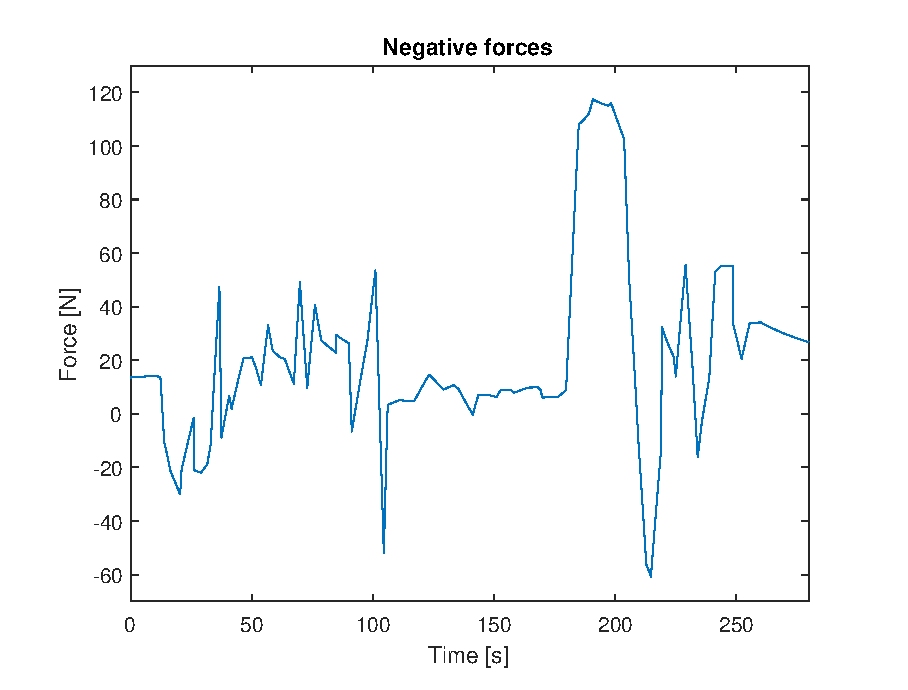
\includegraphics[width=0.5\textwidth]{./img/testrig_negative_forces.eps}
    \caption{Negative forces acting upon Elba in one lap.}
\end{figure}

Torque required on wheel of ELBA:$$T_w = F_n\*r_w$$

Torque required for roller on test rig: $$T_r = \frac{T_w\*r_r}{r_w}$$

Required torque for motor, $T_m$: $$T_m = T_t + J_r\*\ddot{\phi} + d\*\dot{\phi}_m + k\*\phi_m$$

Power required for motor: $$P_m = T_m\*\dot{\phi}_m$$

The inertia $J_r$ for the rollers on the testrig was calculated to be $0.0039$ $kgm^2$

This results in $P_m = 1000$ W

\begin{figure}[H]
    \label{fig:testrig_power_required}
    \centering
    \includegraphics[width=0.5\textwidth]{./img/testrig_power_required.eps}
    \caption{Power required for the motor on the testrig.}
\end{figure}
